\documentclass{standalone}
\usepackage{mintikz}

\pgfdeclarelayer{background}
\pgfdeclarelayer{foreground}
\pgfsetlayers{background,main,foreground}
\usepackage{pifont}% http://ctan.org/pkg/pifont
\newcommand{\cmark}{\ding{51}}%
\newcommand{\xmark}{\ding{55}}%

\begin{document}
\thispagestyle{empty}
\begin{tikzpicture}[]
    \tikzset{header/.style={font={\Large\bfseries}, rounded corners, fill=#1!0},
        header/.default={gray},
        subheader/.style={draw, rounded corners, fill=#1!0},
        subheader/.default={gray},
    }
    % Start top
    \begin{scope}[local bounding box=HOSTBOX, yshift=0cm]
        %%%%%%%%%%%%%%%%%%%%%%%%%%%%%%%%%%%%%%%%%%%%%%%%%%%%%%%%%%%%%%%%%%%%%%%
        % Start PRIOR
        \node[header=black, minimum width=10cm]
            (HOSTHEAD) at (5,0) {CR\'EATION HOSTLIB};
        %%%%%%%%%%%%%%%%%%%%%%%%%%%%%%%%%%%%%%%%%%%%%%%%%%%%%%%%%%%%%%%%%%%%%%%
        % M DIST from BP_lowz HOSTLIB
        \pgfplotstableread{../data/mdist.txt}{\mtable}
        \begin{axis}[name=mdist, scale=0.3,
            yshift=-1cm, anchor=north,
            xmin=6, xmax=14,
            ymin=0, ymax=0.6,
            xlabel=$M$, ylabel=$P$,
            axis lines=left,
            clip=false]
            \addplot[smooth, black]
                table[x=M, y=P] from \mtable;
        \end{axis}
        %%%%%%%%%%%%%%%%%%%%%%%%%%%%%%%%%%%%%%%%%%%%%%%%%%%%%%%%%%%%%%%%%%%%%%%
        % X1 DIST from basemodel
        \pgfplotstableread{../data/basemodel.txt}{\basetable}
        \begin{axis}[name=x1dist, scale=0.3,
            at={(mdist.below south west)}, yshift=-0.3cm, anchor=north west,
            xmin=-3, xmax=3,
            ymin=0, ymax=0.5,
            xlabel=$\bar{x_1}$, ylabel=$P$,
            axis lines=left,
            clip=false]
            \addplot[smooth, black]
                table[x=xlin, y=values] from \basetable;
        \end{axis}
        %%%%%%%%%%%%%%%%%%%%%%%%%%%%%%%%%%%%%%%%%%%%%%%%%%%%%%%%%%%%%%%%%%%%%%%
        % c DIST from stretchevol's asym with Scolnic 18 params:
        % -0.068, 0.034, 0.123
        \pgfplotstableread{../data/casym.txt}{\ctable}
        \begin{axis}[name=cdist, scale=0.3,
            at={(x1dist.below south west)}, yshift=-0.3cm, anchor=north west,
            xmin=-0.3, xmax=0.3,
            ymin=0, ymax=5,
            xlabel=$\bar{c}$, ylabel=$P$,
            axis lines=left,
            clip=false]
            \addplot[smooth, black]
                table[x=clin, y=values] from \ctable;
        \end{axis}
        %%%%%%%%%%%%%%%%%%%%%%%%%%%%%%%%%%%%%%%%%%%%%%%%%%%%%%%%%%%%%%%%%%%%%%%
        % START HOSTLIB
        \matrix[matrix of nodes, anchor=west,
            row sep=-1pt, column sep=-\pgflinewidth,
            text width=40pt, align=center,
            %left delimiter=|,
            nodes={anchor=center, align=center}]
            (Mhostlib) at ([shift={(1, 0)}]x1dist.east)
            {ID & $z$ & $M_*$ & $x_1$ & $c$ & $\Delta$mag \\
            \vdots & \vdots & \vdots & \vdots & \vdots & \vdots\\
            \vdots & \vdots & \vdots & \vdots & \vdots & \vdots\\
            \vdots & \vdots & \vdots & \vdots & \vdots & \vdots\\
            \vdots & \vdots & \vdots & \vdots & \vdots & \vdots\\
            \vdots & \vdots & \vdots & \vdots & \vdots & \vdots\\
            \vdots & \vdots & \vdots & \vdots & \vdots & \vdots\\
            \vdots & \vdots & \vdots & \vdots & \vdots & \vdots\\
            \vdots & \vdots & \vdots & \vdots & \vdots & \vdots\\
            \vdots & \vdots & \vdots & \vdots & \vdots & \vdots\\};
        % Vlines
        \foreach \n in {1, 3, 4, 5}{
        \draw[]
            (Mhostlib-1-\n.north east-|Mhostlib-10-\n.south east) |-
        (Mhostlib-10-\n.south east);}
        \draw[]
            (Mhostlib-2-2.north east-|Mhostlib-10-2.south east) |-
            (Mhostlib-10-2.south east);
        % HOSTLIB z to hostmass
        \draw[->, >=Stealth]
            ([shift={(-10pt,0)}]Mhostlib-1-2.east) --
            ([shift={(+10pt,0)}]Mhostlib-1-3.west);
        % HEADER
        \node[subheader=black, above]
            (HOSTLIB) at (Mhostlib.north) {HOSTLIB};
        %%%%%%%%%%%%%%%%%%%%%%%%%%%%%%%%%%%%%%%%%%%%%%%%%%%%%%%%%%%%%%%%%%%%%%%
        % DIST to HOSTLIB
        \foreach \d/\y in {mdist/0.2, x1dist/0, cdist/-0.2}{
            \draw[->, >=Stealth]
                (\d.east) --++ (0.6,0) |-
            ([shift={(-0.2,0)}]Mhostlib.west) --
            (Mhostlib.west);}
    \end{scope}
    \begin{pgfonlayer}{background}
        \draw[fill=black!10, rounded corners]
        ([shift={(0, -2pt)}]HOSTBOX.north east |- HOSTHEAD.south east) --
            %node (HOSTNUM) {} --
        ([shift={(0, -2pt)}]HOSTBOX.north west |- HOSTHEAD.south west) --
            (HOSTBOX.south west) --
            (HOSTBOX.south east)
            node[inner sep=0] (HOSTNUM) {} -- cycle ;
        \node[above left, scale=2, draw, rounded corners]
            at (HOSTNUM.center) {2};
        % \path (HOSTBOX.north west) -- node[midway, black!10, scale=20]
        %     {2} (HOSTBOX.south east);
    \end{pgfonlayer}
    %%%%%%%%%%%%%%%%%%%%%%%%%%%%%%%%%%%%%%%%%%%%%%%%%%%%%%%%%%%%%%%%%%%%%%%%%%%
    % Start left
    %%%%%%%%%%%%%%%%%%%%%%%%%%%%%%%%%%%%%%%%%%%%%%%%%%%%%%%%%%%%%%%%%%%%%%%%%%%
    \begin{scope}[local bounding box=TIRAGEBOX,
        shift={($(HOSTBOX.south west)+(0cm,-0.5cm)$)}]%yshift=0cm]
        %%%%%%%%%%%%%%%%%%%%%%%%%%%%%%%%%%%%%%%%%%%%%%%%%%%%%%%%%%%%%%%%%%%%%%%
        % Start TIRAGE
        \node[header=orchid, minimum width=5cm] (TIRAGEHEAD) at (0,0) {TIRAGE};
        %%%%%%%%%%%%%%%%%%%%%%%%%%%%%%%%%%%%%%%%%%%%%%%%%%%%%%%%%%%%%%%%%%%%%%%
        % WGTMAP
        \pgfplotstableread{../data/SDSS.txt}{\wgttable}
        \node[subheader=black, below=0.2cm]
            (WEIGHTMAP) at (TIRAGEHEAD.south) {WEIGHTMAP};
        \begin{axis}[name=Mwgt, scale=0.7,
            at={(WEIGHTMAP.south west)}, yshift=-0.2cm, anchor=north,
            %shift={($(WEIGHTMAP.south)+(0,-0.4cm)$)}, anchor=north,
            xmin=8, xmax=12.3,
            ymin=0, ymax=1,
            xlabel=$M_*$, ylabel=$P(M)$,
            axis lines=left,
            clip=true]
            \addplot[black, samples=500]
                table[x=M, y=WGT] from \wgttable;
        \end{axis}
        %%%%%%%%%%%%%%%%%%%%%%%%%%%%%%%%%%%%%%%%%%%%%%%%%%%%%%%%%%%%%%%%%%%%%%%
        % Add space
        \node[minimum width=8.6cm] (SPACE) at (Mwgt.south east) {} ;
        %%%%%%%%%%%%%%%%%%%%%%%%%%%%%%%%%%%%%%%%%%%%%%%%%%%%%%%%%%%%%%%%%%%%%%%
        % z DIST Rate from equation 6 of DES 2019
        % https://arxiv.org/pdf/1811.02379.pdf
        \node[subheader=black, below=5.5cm, anchor=north]
            (ZDIST) at (WEIGHTMAP.south) {Distribution des redshifts};
        \begin{axis}[name=zdist, scale=0.7,
            at={(Mwgt.below south west)}, yshift=-1cm, anchor=north west,
            xmin=0, xmax=1.2,
            ymin=0, ymax=11,
            xlabel=$\bar{z}$, ylabel=\# (1$^{-15}$) \si{an^{-1}Mpc^{-3}},
            axis lines=left,
            clip=true]
            % \addplot[smooth, black]
            %     {1.75*(1+x)^2.11};
            \addplot[smooth, black]
                {2.6*(1+x)^2.2};
        \end{axis}
        %%%%%%%%%%%%%%%%%%%%%%%%%%%%%%%%%%%%%%%%%%%%%%%%%%%%%%%%%%%%%%%%%%%%%%%
        % \begin{pgfonlayer}{background}
        %     \node[gray!20, scale=20, inner sep=0] (TIRAGEBOX.south) {1};
        % \end{pgfonlayer}
    \end{scope}
    %%%%%%%%%%%%%%%%%%%%%%%%%%%%%%%%%%%%%%%%%%%%%%%%%%%%%%%%%%%%%%%%%%%%%%%%%%%
    % Show tirage
    \draw[Orchid, thick]
        ([shift={(0,-6pt)}]Mhostlib-9-1.north west) node [] (topleft) {}--
        (Mhostlib-9-1.south west) node [] (bottomleft) {} --
        (Mhostlib-9-6.south east) node [] (bottomright) {} --
        ([shift={(0,-6pt)}]Mhostlib-9-6.north east) --
        cycle ;
    % Wgt and Z to HOSTLIB
    \draw[dashed, Orchid, ->, >=Stealth]
        (Mwgt.east) -|
            node [right=0.15cm, font=\bfseries,
                  anchor=north, rotate=90] {Lien avec l'environnement}
        (bottomleft);
    \draw[dashed, Orchid, ->, >=Stealth]
        (zdist.east) -| (bottomleft);
    %%%%%%%%%%%%%%%%%%%%%%%%%%%%%%%%%%%%%%%%%%%%%%%%%%%%%%%%%%%%%%%%%%%%%%%%%%%
    \begin{scope}[local bounding box=SIMBOX, anchor=north west,
        shift={($(TIRAGEBOX.north east)+(5cm,0)$)}]
        %%%%%%%%%%%%%%%%%%%%%%%%%%%%%%%%%%%%%%%%%%%%%%%%%%%%%%%%%%%%%%%%%%%%%%%
        % Start TRUE
        \node[header=cornflowerblue, minimum width=5cm, anchor=north]
            (SIMHEAD) at (2.5,0) {INSTRUMENT};
            % (SIMHEAD) at (2.5,0) {SIMULATION};
        % Start timeseries
        \node[anchor=north west] (TS) at
            ([shift={(-6.5cm,-1cm)}]SIMHEAD.center)
            %([shift={(3cm,-1cm)}]SIMBOX.north west)
            {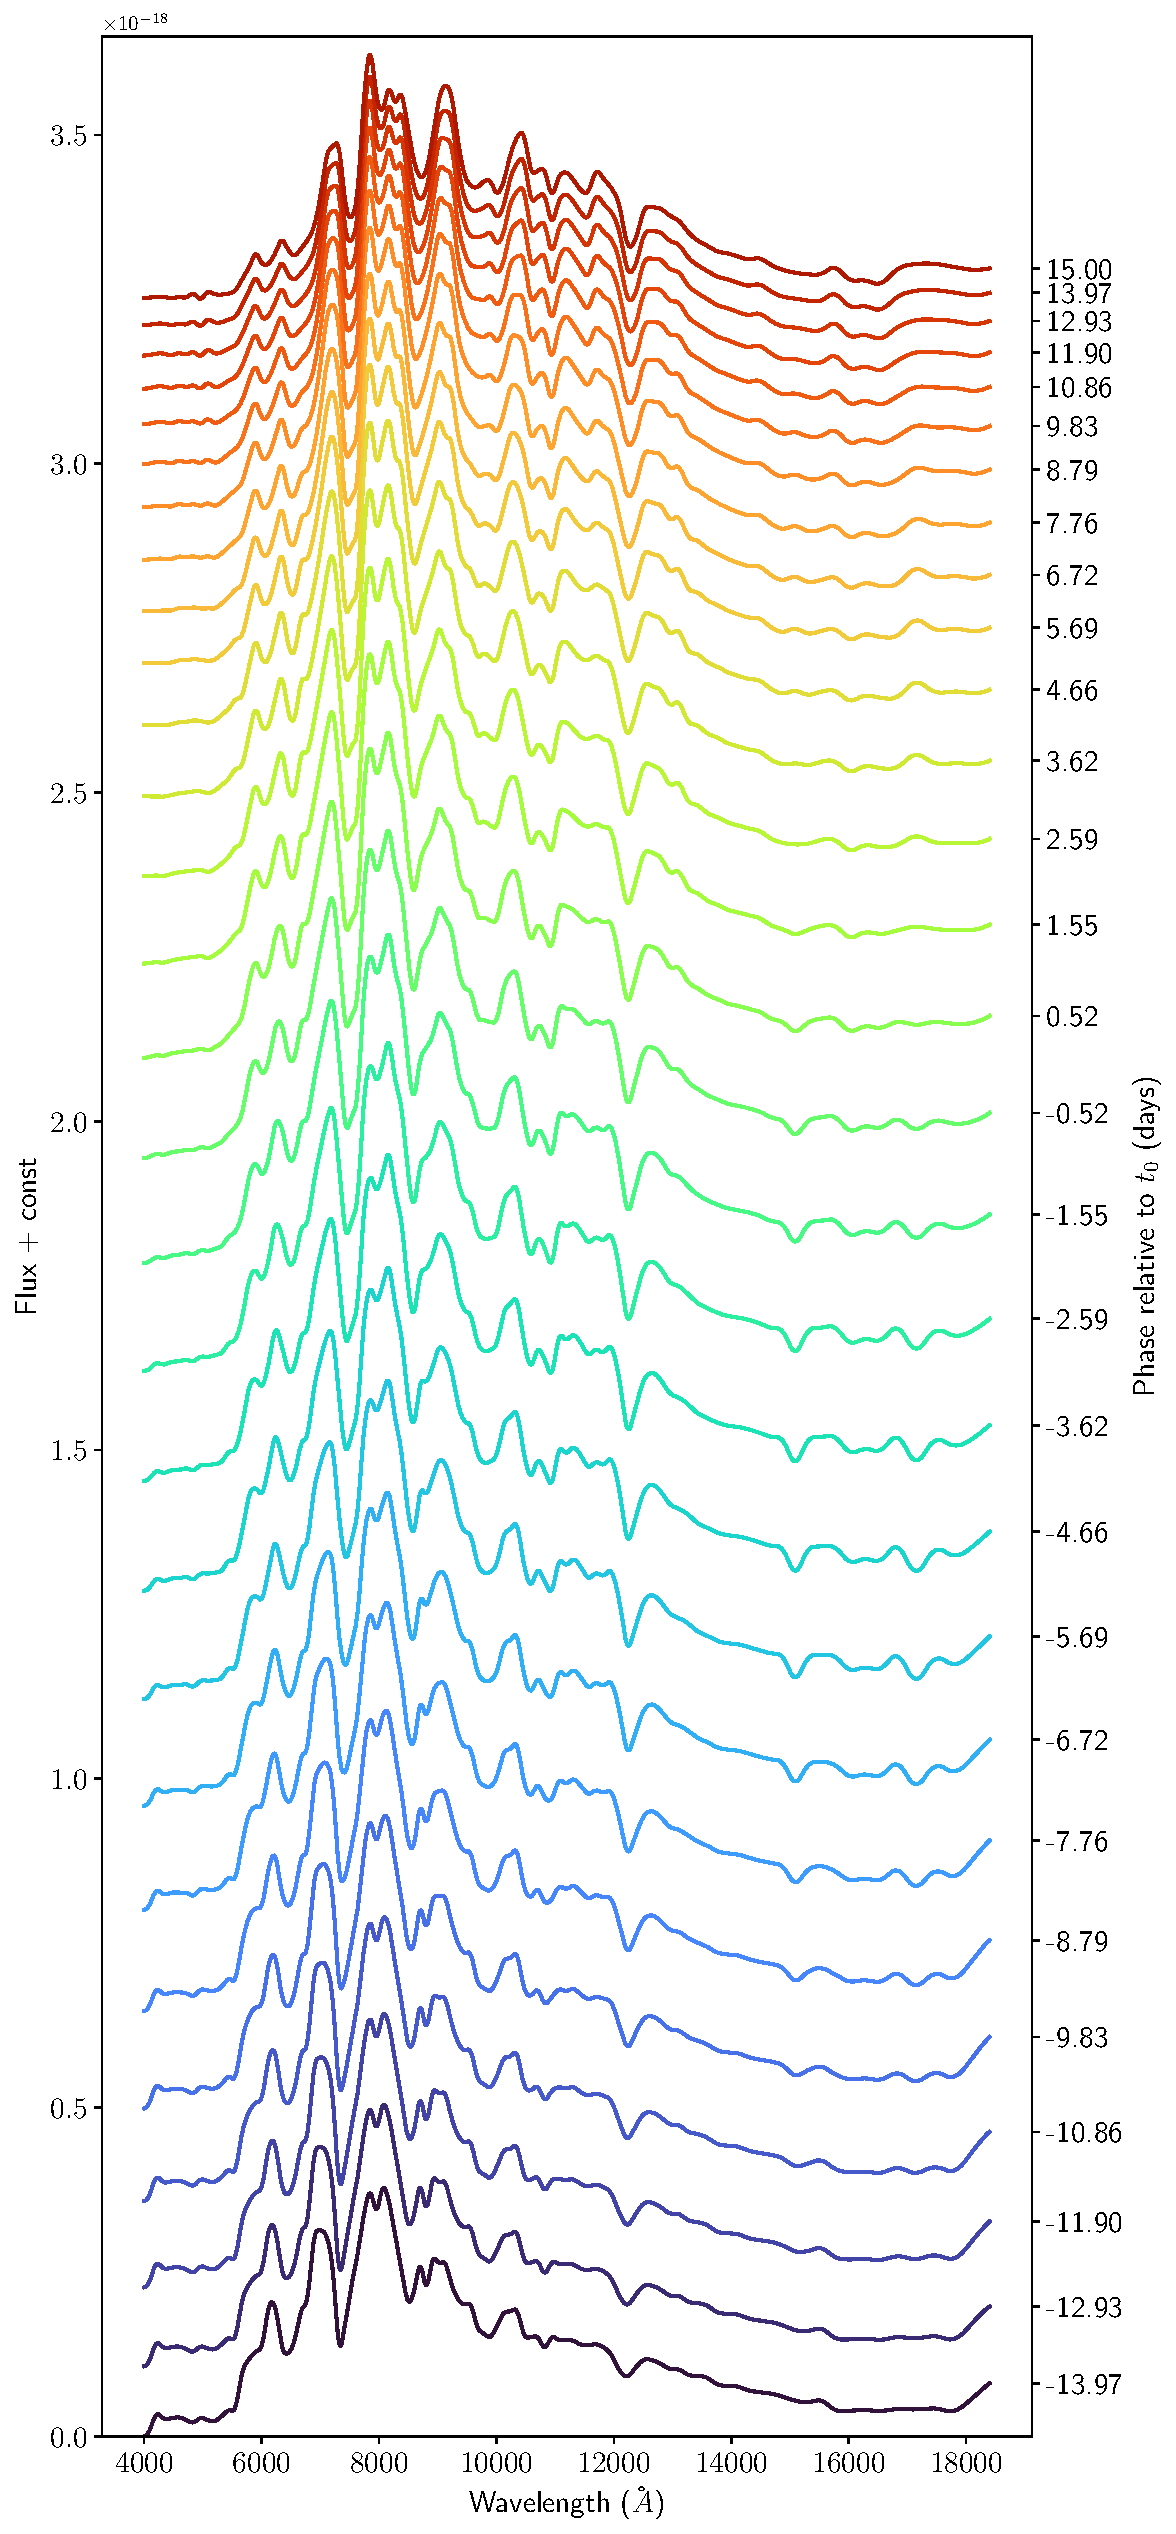
\includegraphics[scale=0.25]{timeseries.pdf}};
        \node[anchor=west, right, thick, scale=3] (plus) at
            ([shift={(-.2cm,0)}]TS.east) {$\otimes$};
        %%%%%%%%%%%%%%%%%%%%%%%%%%%%%%%%%%%%%%%%%%%%%%%%%%%%%%%%%%%%%%%%%%%%%%%
        % SIMBLIB
        \matrix[matrix of nodes, anchor=west,
            row sep=-1pt, column sep=-\pgflinewidth,
            text width=25pt, align=center,
            %left delimiter=|,
            nodes={anchor=center, font=\footnotesize, align=center}]
            (Msimlib) at ([shift={(-0.7cm,0)}]plus.east)
            {MJD & FLT & CCD & PSF & $\cdots$ \\
            \vdots & \vdots & \vdots & \vdots & \vdots\\
            \vdots & \vdots & \vdots & \vdots & \vdots\\
            \vdots & \vdots & \vdots & \vdots & \vdots\\
            \vdots & \vdots & \vdots & \vdots & \vdots\\
            \vdots & \vdots & \vdots & \vdots & \vdots\\};
        % Vlines
        \foreach \n in {1, 2, 3, 4}{
        \draw[]
            (Msimlib-1-\n.north east-|Msimlib-6-\n.south east) |-
        (Msimlib-6-\n.south east);}
        % HEADER
        \node[subheader=black, above=.2cm]
            (SIMLIB) at (Msimlib.north) {SIMLIB};
        %%%%%%%%%%%%%%%%%%%%%%%%%%%%%%%%%%%%%%%%%%%%%%%%%%%%%%%%%%%%%%%%%%%%%%%
        % Bands and LC
        \node[anchor=north] (TSDSS) at ([shift={(.5cm,0cm)}]TS.south)
            {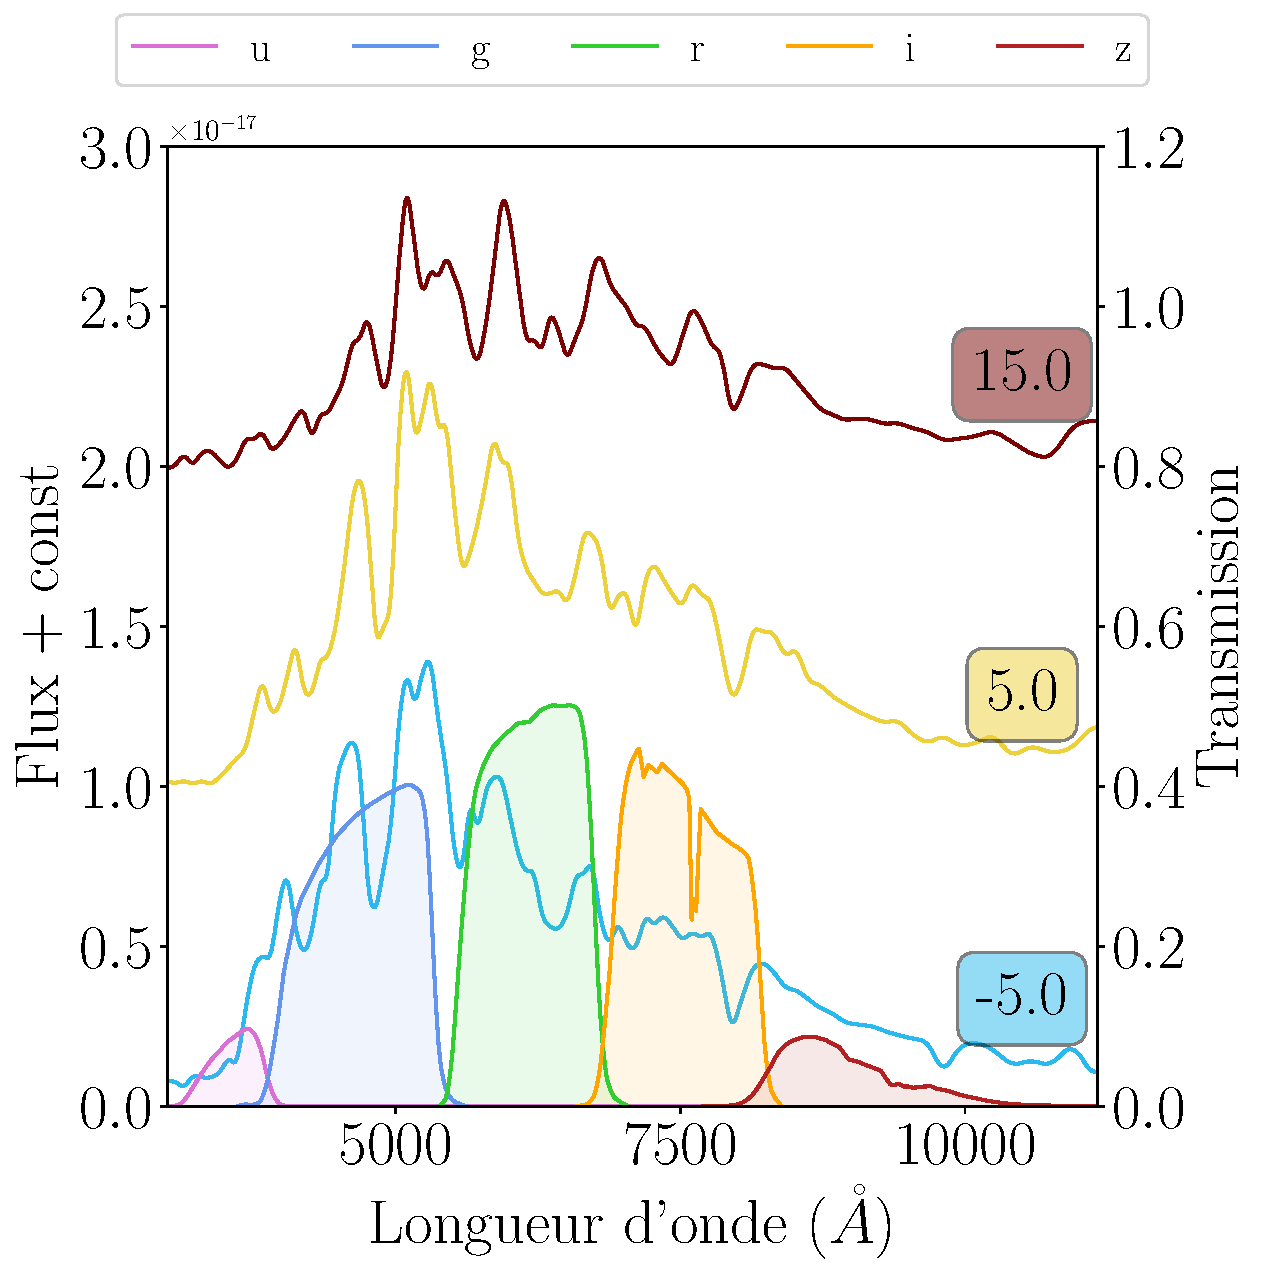
\includegraphics[width=5cm]{timeseries_sdss.pdf}};
        \node[anchor=west] (SDLC) at ([shift={(.5cm,0)}]TSDSS.east)
            {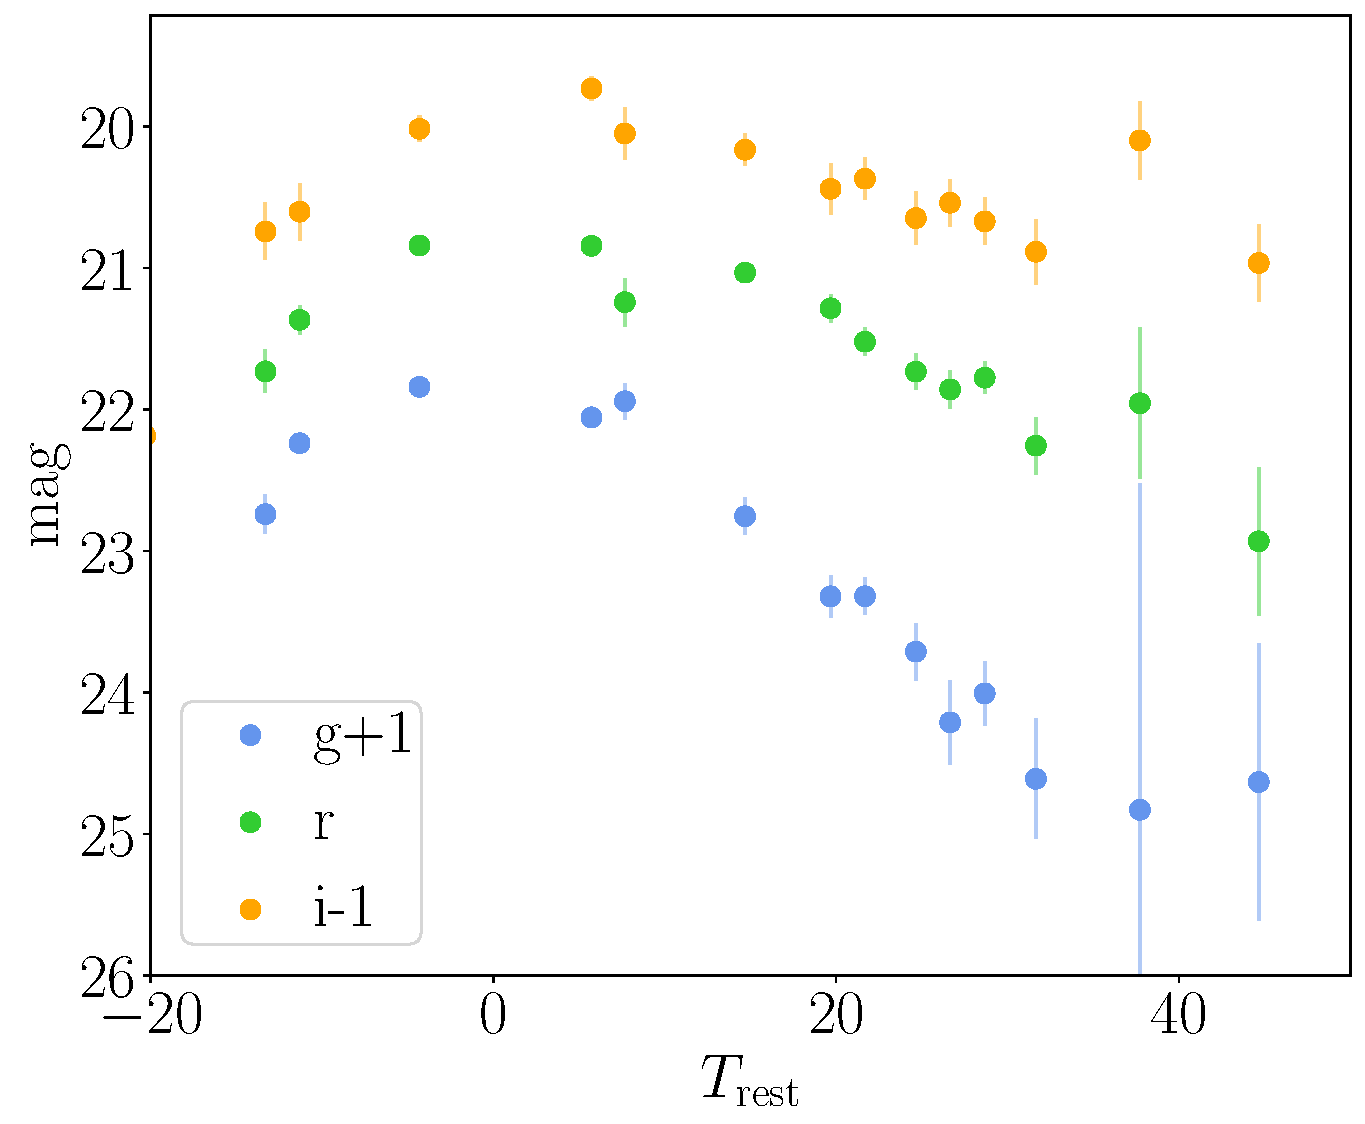
\includegraphics[width=5cm]{lc_2005gg_NOSALT.pdf}};
        %%%%%%%%%%%%%%%%%%%%%%%%%%%%%%%%%%%%%%%%%%%%%%%%%%%%%%%%%%%%%%%%%%%%%%%
        \draw[rounded corners]
            (TS.north west) node [right=2cm, inner sep=0] (tosim) {} --
            (TS.south west) node [right] (corner) {} --
            (TS.south east -| Msimlib.south east) --
            (Msimlib.north east |- TS.north east) -- cycle;
        %%%%%%%%%%%%%%%%%%%%%%%%%%%%%%%%%%%%%%%%%%%%%%%%%%%%%%%%%%%%%%%%%%%%%%%
        % Arrows
            \draw[thick, ->, >=Stealth] ([shift={(0.3cm,0)}]corner.south west) |- (TSDSS.west) ;
        \draw[->, >=Stealth] (TSDSS.east) -- (SDLC.west);
    \end{scope}
    %%%%%%%%%%%%%%%%%%%%%%%%%%%%%%%%%%%%%%%%%%%%%%%%%%%%%%%%%%%%%%%%%%%%%%%
    % Point to sim
    \draw[dashed, cornflowerblue, ->, >=Stealth]
        (bottomright) --
        (bottomright |- cdist.south east) --
            node [midway, below, font=\bfseries] {G\'en\'eration}
        (tosim |- cdist.south east) --
        (tosim) ;
    %%%%%%%%%%%%%%%%%%%%%%%%%%%%%%%%%%%%%%%%%%%%%%%%%%%%%%%%%%%%%%%%%%%%%%%
    \begin{pgfonlayer}{background}
        \draw[fill=orchid!20, rounded corners]
        ([shift={(0, -2pt)}]TIRAGEBOX.north east |- TIRAGEHEAD.south east) --
            %node (TIRAGENUM) {} --
        ([shift={(0, -2pt)}]TIRAGEBOX.north west |- TIRAGEHEAD.south west) --
        (TIRAGEBOX.south west |- SIMBOX.south west) --
        (TIRAGEBOX.south east |- SIMBOX.south east) node (TIRAGENUM) {} --
        cycle ;
        % \path (TIRAGEBOX.north west) -- node[midway, black!10, scale=20]
        %     {1} (TIRAGEBOX.south east);
        \node[above left, scale=2, draw, rounded corners]
            at (TIRAGENUM.center) {1};
    \end{pgfonlayer}
    \begin{pgfonlayer}{background}
        \draw[fill=cornflowerblue!10, rounded corners]
        ([shift={(0, -2pt)}]SIMBOX.north east |- SIMHEAD.south east) --
            %node (SIMNUM) {} --
        ([shift={(0, -2pt)}]SIMBOX.north west |- SIMHEAD.south west) --
        (SIMBOX.south west) node (SIMNUM) {} --
        (SIMBOX.south east) --
        cycle ;
        % \path (SIMBOX.north west) -- node[midway, black!10, scale=20]
        %     {3} (SIMBOX.south east);
        \node[above right, scale=2, draw, rounded corners]
            at (SIMNUM.center) {3};
    \end{pgfonlayer}
    %%%%%%%%%%%%%%%%%%%%%%%%%%%%%%%%%%%%%%%%%%%%%%%%%%%%%%%%%%%%%%%%%%%%%%%
    \begin{scope}[local bounding box=SELBOX, anchor=north west,
        shift={($(TIRAGEBOX.south west|-SIMBOX.south west)+(-0.35cm,-0.3cm)$)}]
        % Start SELECTION
        \node[header=limegreen, minimum width=5cm]
            (SELHEAD) at (2.9,0) {S\'ELECTION};
        %%%%%%%%%%%%%%%%%%%%%%%%%%%%%%%%%%%%%%%%%%%%%%%%%%%%%%%%%%%%%%%%%%%%%%%
        % Start SPECSEL
        \node[subheader=black, anchor=north]
            (SPECSEL) at ([shift={(0,-0.5cm)}]SELHEAD.south) {D\'etection};
        % SDSS SPECEFF from sdss spec
        \pgfplotstableread{../data/sdss_spec.dat}{\sdspectable}
        \findMax{\sdspectable}{r}{\rmax}
        \begin{axis}[name=sdspec, scale=0.8,
            at={(SPECSEL.south)}, anchor=north,
            % yshift=-1cm, xshift=-1cm,
            xmin=16.0, xmax=\rmax*0.8,
            ymin=0, ymax=1.0,
            xlabel=$r$ (mag), ylabel=\'Efficacit\'e spectroscopique,
            axis lines=left,
            clip=true]
            \addplot[black, smooth]
                table[x=r, y=SPECEFF] from \sdspectable;
        \end{axis}
        %%%%%%%%%%%%%%%%%%%%%%%%%%%%%%%%%%%%%%%%%%%%%%%%%%%%%%%%%%%%%%%%%%%%%%%
        % Start PHOTSEL
        \node[subheader=black, anchor=north]
            (PHOTSEL) at ([shift={(0,-6.0cm)}]SPECSEL.south) {Coupes de
            qualit\'e};
        \matrix[matrix of nodes, anchor=north,
            row sep=-1pt, column sep=-\pgflinewidth,
            text width=50pt, align=center,
            %left delimiter=|,
            nodes={anchor=center, font=\footnotesize, align=center}]
            (PHOTLIST) at ([shift={(0,-0.2cm)}]PHOTSEL.south)
            {$T_{\rm rest} < 0$ & $T_{\rm rest} > 10$
                                & SNR > 5 $gri$
                                & $-3 < x_1 < 3$ & $\cdots$\\
                \cmark & \xmark & \xmark & \xmark & $\cdots$ \\
                \cmark & \cmark & \cmark & \xmark & $\cdots$ \\
                \xmark & \xmark & \cmark & \xmark & $\cdots$ \\
                \cmark & \cmark & \cmark & \cmark & $\cdots$ \\
                \vdots & \vdots & \vdots & \vdots & \vdots \\};
        % Vlines
        \foreach \n in {1, 2, 3, 4}{
        \draw[]
            (PHOTLIST-1-\n.north east-|PHOTLIST-6-\n.south east) |-
        (PHOTLIST-6-\n.south east);}
        % Draw detected
        \draw[limegreen, thick]
            (PHOTLIST-3-1.north west) node [] (topleft) {}--
            (PHOTLIST-3-1.south west) node [] (bottomleft) {} --
            (PHOTLIST-3-5.south east |- PHOTLIST-3-1.south west)
                node [] (bottomrightv) {} --
                node [midway, right=0.2] (rightv) {}
            (PHOTLIST-3-5.north east |- PHOTLIST-3-1.north west)
                node [left=0.2] (toprightv) {} --
            cycle ;
        % Draw ajusted
        \draw[orange, thick]
            (PHOTLIST-5-1.north west) node [] (topleft) {}--
            (PHOTLIST-5-1.south west) node [] (bottomleft) {} --
            (PHOTLIST-5-5.south east |- PHOTLIST-5-1.south west)
                node [] (bottomrighto) {} --
                node [midway, inner sep=0] (righto) {}
            (PHOTLIST-5-5.north east |- PHOTLIST-5-1.north west)
                node [left=0.2] (toprighto) {} --
            cycle ;
    \end{scope}
    %%%%%%%%%%%%%%%%%%%%%%%%%%%%%%%%%%%%%%%%%%%%%%%%%%%%%%%%%%%%%%%%%%%%%%%
    \begin{scope}[local bounding box=CONSBOX, anchor=north west,
        shift={($(SIMBOX.south west)+(1.75cm,-0.3cm)$)}]
        %shift={($(SELBOX.north east)+(1.3cm,0)$)}]
    %%%%%%%%%%%%%%%%%%%%%%%%%%%%%%%%%%%%%%%%%%%%%%%%%%%%%%%%%%%%%%%%%%%%%%%
        % Start CONS
        \node[header=orange, minimum width=5cm, anchor=north]
            (CONSHEAD) at (5,0) {CONSERV\'E};
        %%%%%%%%%%%%%%%%%%%%%%%%%%%%%%%%%%%%%%%%%%%%%%%%%%%%%%%%%%%%%%%%%%%%%%%
        % M DIST from dumps and 2_LCFIT
        \pgfplotstableread{../data/mTrue.txt}{\mtrue}
        \pgfplotstableread{../data/mSelected.txt}{\msel}
        \pgfplotstableread{../data/mFitted.txt}{\mfit}
        \begin{axis}[name=mdump, scale=0.7,
            at={(CONSHEAD.center)},
            xshift=-5.5cm, yshift=-1.5cm, anchor=north west,
            xmin=7, xmax=12.1,
            ymin=0, ymax=0.73,
            xlabel=$M$, ylabel=$P$,
            axis lines=left,
            legend pos=north west,
            legend columns=3,
            legend style={anchor=center, at={(1.15, 1.2)}},
            clip=false]
            \addplot[samples=500, Orchid, line width=1pt]
                table[x=mlin, y=values] from \mtrue;
            \addlegendentry{Test\'e}
            \addplot[samples=500, limegreen, line width=1pt]
                table[x=mlin, y=values] from \msel;
            \addlegendentry{D\'etect\'e}
            \addplot[samples=500, orange, line width=1pt]
                table[x=mlin, y=values] from \mfit;
            \addlegendentry{Ajust\'e}
        \end{axis}
        %%%%%%%%%%%%%%%%%%%%%%%%%%%%%%%%%%%%%%%%%%%%%%%%%%%%%%%%%%%%%%%%%%%%%%%
        % C DIST dumps and 2_LCFIT
        \pgfplotstableread{../data/cTrue.txt}{\ctrue}
        \pgfplotstableread{../data/cSelected.txt}{\csel}
        \pgfplotstableread{../data/cFitted.txt}{\cfit}
        \begin{axis}[name=cdump, scale=0.7,
            at={(mdump.below south west)},
            yshift=-0.3cm, anchor=north west,
            xmin=-0.3, xmax=0.5,
            ymin=0, ymax=7.2,
            xlabel=$c$, ylabel=$P$,
            axis lines=left,
            legend pos=north west,
            clip=false]
            \addplot[samples=500, Orchid, line width=1pt]
                table[x=clin, y=values] from \ctrue;
            % \addlegendentry{V\'erit\'e}
            \addplot[samples=500, limegreen, line width=1pt]
                table[x=clin, y=values] from \csel;
            % \addlegendentry{S\'electionn\'e}
            \addplot[samples=500, orange, line width=1pt]
                table[x=clin, y=values] from \cfit;
            % \addlegendentry{Ajust\'e}
        \end{axis}
        %%%%%%%%%%%%%%%%%%%%%%%%%%%%%%%%%%%%%%%%%%%%%%%%%%%%%%%%%%%%%%%%%%%%%%%
        % Z DIST dumps and 2_LCFIT
        \pgfplotstableread{../data/zTrue.txt}{\ztrue}
        \findMax{\ztrue}{zlin}{\zxmax}
        \findMax{\ztrue}{values}{\zymax}
        \pgfplotstableread{../data/zSelected.txt}{\zsel}
        \pgfplotstableread{../data/zFitted.txt}{\zfit}
        \begin{axis}[name=zdump, scale=0.7,
            at={(cdump.right of north east)},
            anchor=left of north west,
            xmin=0, xmax=\zxmax,
            ymin=0, ymax=\zymax,
            xlabel=$z$, ylabel=$P$,
            axis lines=left,
            legend pos=north west,
            clip=false]
            \addplot[samples=500, Orchid, line width=1pt]
                table[x=zlin, y=values] from \ztrue;
            % \addlegendentry{V\'erit\'e}
            \addplot[samples=500, limegreen, line width=1pt]
                table[x=zlin, y=values] from \zsel;
            % \addlegendentry{S\'electionn\'e}
            \addplot[samples=500, orange, line width=1pt]
                table[x=zlin, y=values] from \zfit;
            % \addlegendentry{Ajust\'e}
        \end{axis}
        %%%%%%%%%%%%%%%%%%%%%%%%%%%%%%%%%%%%%%%%%%%%%%%%%%%%%%%%%%%%%%%%%%%%%%%
        % X1 DIST dumps and 2_LCFIT
        \pgfplotstableread{../data/xTrue.txt}{\xtrue}
        \pgfplotstableread{../data/xSelected.txt}{\xsel}
        \pgfplotstableread{../data/xFitted.txt}{\xfit}
        \begin{axis}[name=xdump, scale=0.7,
            at={(mdump.north east -| zdump.west)},
            anchor=north west,
            xmin=-3, xmax=3,
            ymin=0, ymax=0.5,
            xlabel=$x_1$, ylabel=$P$,
            axis lines=left,
            legend pos=north west,
            clip=false]
            \addplot[samples=500, Orchid, line width=1pt]
                table[x=xlin, y=values] from \xtrue;
            % \addlegendentry{V\'erit\'e}
            \addplot[samples=500, limegreen, line width=1pt]
                table[x=xlin, y=values] from \xsel;
            % \addlegendentry{S\'electionn\'e}
            \addplot[samples=500, orange, line width=1pt]
                table[x=xlin, y=values] from \xfit;
            % \addlegendentry{Ajust\'e}
        \end{axis}
        %%%%%%%%%%%%%%%%%%%%%%%%%%%%%%%%%%%%%%%%%%%%%%%%%%%%%%%%%%%%%%%%%%%%%%%
    \end{scope}
    %%%%%%%%%%%%%%%%%%%%%%%%%%%%%%%%%%%%%%%%%%%%%%%%%%%%%%%%%%%%%%%%%%%%%%%
    % Plot orange in PHOT to CONS
    \draw[orange, dashed, ->, >=Stealth] 
        ([shift={(0.1cm,0)}]righto.east) --++ (0.4cm,0) |-
            node [left, rotate=90, font=\bfseries,
                  anchor=east, yshift=-0.3cm] {Ajustement conserv\'e}
        ([shift={(-0.1,-0.2)}]CONSBOX.west);
    % Plot green in PHOT to CONS
    \draw[limegreen, dashed, ->, >=Stealth] 
        (toprightv) |-
            node [left, rotate=90, font=\bfseries,
                  anchor=east, yshift=-0.3cm] {D\'etection rejet\'ee}
        ([shift={(-0.2,0.2)}]CONSBOX.west);
    %%%%%%%%%%%%%%%%%%%%%%%%%%%%%%%%%%%%%%%%%%%%%%%%%%%%%%%%%%%%%%%%%%%%%%%
    \begin{pgfonlayer}{background}
        \draw[fill=orange!20, rounded corners]
            ([shift={(0, -2pt)}]CONSBOX.north east |- CONSHEAD.south east) --
                % node (CONSNUM) {} --
            ([shift={(0, -2pt)}]CONSBOX.north west |- CONSHEAD.south west)
                node (CONSNUM) {} --
            (CONSBOX.south west) --
            (CONSBOX.south east) --
            cycle ;
        \node[below right, scale=2, draw, rounded corners] at (CONSNUM.center) {5};
        % \path (CONSBOX.north west) -- node[midway, black!10, scale=20]
        %     {5} (CONSBOX.south east);
    \end{pgfonlayer}
    %%%%%%%%%%%%%%%%%%%%%%%%%%%%%%%%%%%%%%%%%%%%%%%%%%%%%%%%%%%%%%%%%%%%%%%
    \begin{pgfonlayer}{background}
        \draw[fill=limegreen!20, rounded corners]
            ([shift={(0, -2pt)}]SELBOX.north east |- SELHEAD.south east)
                node (SELNUM) {} --
            ([shift={(0, -2pt)}]SELBOX.north west |- SELHEAD.south west) --
            (SELBOX.south west |- CONSBOX.south west) --
            (SELBOX.south east |- CONSBOX.south east) --
            cycle ;
        % \path (SELBOX.north west) -- node[midway, black!10, scale=20]
        %     {4} (SELBOX.south east);
        \node[below left, scale=2, draw, rounded corners]
            at (SELNUM.center) {4};
    \end{pgfonlayer}
    %%%%%%%%%%%%%%%%%%%%%%%%%%%%%%%%%%%%%%%%%%%%%%%%%%%%%%%%%%%%%%%%%%%%%%%
    % Point to SEL
    \draw[limegreen, dashed, ->, >={Stealth[scale=1.5]}]
        (SIMBOX.south west) -- (SELNUM.center) ;
\end{tikzpicture}
\end{document}
